\begin{figure}[!t]
\centering
\begin{tikzpicture}
    \begin{customlegend}[legend columns=3,
        legend entries={$K=2$,$K=4$,$K=10$}
        ,
        legend style={at={(0.45,1.05)},anchor=north,draw=none,font=\footnotesize,column sep=0.1cm}]
    \addlegendimage{only marks, line width=0.23mm,mark size=2.3pt,mark=x,color=LightBlue}
    \addlegendimage{only marks, line width=0.23mm,mark size=2.3pt,mark=star,color=Orange}
    \addlegendimage{only marks, line width=0.23mm,mark size=2.3pt,mark=pentagon,color=Green}
    \end{customlegend}
\end{tikzpicture}
\\[-\lineskip]

\subfloat[$\clen=1200$]{
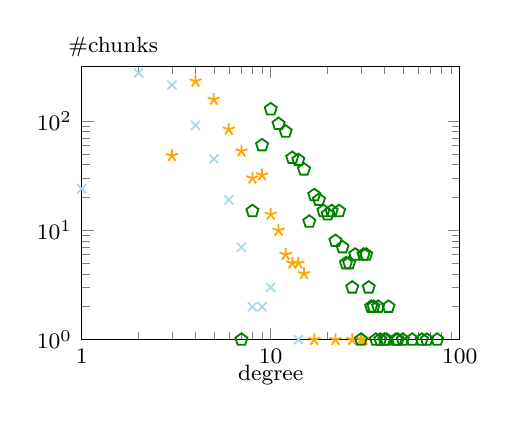
\begin{tikzpicture}[scale=1]
    \begin{axis}[
        height=\columnwidth/2.4,
        width=\columnwidth/1.9,
        ylabel={\#chunks},
        xlabel={degree},
        xmode=log, ymode=log,
        xmin=1, xmax=100,
        ymin=1, ymax=316,
        xtick={1, 10, 100},
        xticklabels={1, 10, 100},
        ytick={1, 10, 100},
        yticklabels={$10^0$, $10^1$, $10^2$},
        every axis y label/.style={at={(current axis.north west)},right=4mm,above=0mm},
        label style={font=\footnotesize},
        tick label style={font=\footnotesize},
        every axis x label/.style={at={(current axis.south)},right=0mm,above=-7mm},
        label style={font=\footnotesize},
        tick label style={font=\footnotesize},
    ]


    \addplot[only marks, mark size=2.3pt, mark=x,color=LightBlue, line width=0.23mm]
        plot coordinates { % SkeTRAG
(1, 24)
(2, 275)
(3, 213)
(4, 91)
(5, 45)
(6, 19)
(7, 7)
(8, 2)
(9, 2)
(10, 3)
(14, 1)
    };

    \addplot[only marks, mark size=2.3pt, mark=star,color=Orange, line width=0.23mm]
        plot coordinates { % SkeTRAG
(3, 48)
(4, 231)
(5, 157)
(6, 84)
(7, 53)
(8, 30)
(9, 32)
(10, 14)
(11, 10)
(12, 6)
(13, 5)
(14, 5)
(15, 4)
(17, 1)
(22, 1)
(27, 1)
(30, 1)
(31, 1)
    };

    \addplot[only marks, mark size=2.3pt, mark=pentagon,color=Green, line width=0.23mm]
        plot coordinates { % SkeTRAG
(7, 1)
(8, 15)
(9, 60)
(10, 128)
(11, 94)
(12, 80)
(13, 46)
(14, 44)
(15, 36)
(16, 12)
(17, 21)
(18, 19)
(19, 15)
(20, 14)
(21, 15)
(22, 8)
(23, 15)
(24, 7)
(25, 5)
(26, 5)
(27, 3)
(28, 6)
(30, 1)
(31, 6)
(32, 6)
(33, 3)
(34, 2)
(35, 2)
(36, 1)
(37, 2)
(38, 1)
(40, 1)
(41, 1)
(42, 2)
(46, 1)
(47, 1)
(50, 1)
(56, 1)
(63, 1)
(67, 1)
(76, 1)
    };

    \end{axis}

\end{tikzpicture}
}%
\hspace{2mm}
\subfloat[$\clen=150$]{
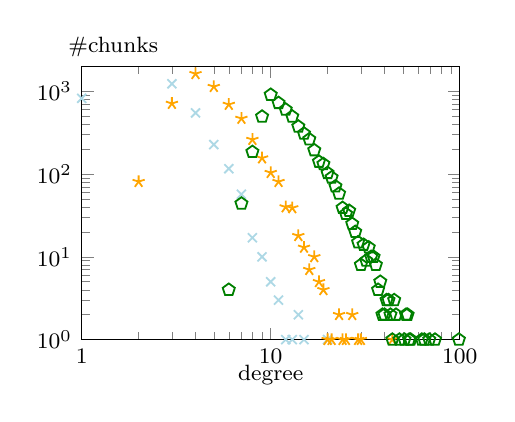
\begin{tikzpicture}[scale=1]
    \begin{axis}[
        height=\columnwidth/2.4,
        width=\columnwidth/1.9,
        ylabel={\#chunks},
        xlabel={degree},
        xmode=log, ymode=log,
        xmin=1, xmax=100,
        ymin=1, ymax=2000,
        xtick={1, 10, 100},
        xticklabels={1, 10, 100},
        ytick={1, 10, 100, 1000},
        yticklabels={$10^0$, $10^1$, $10^2$, $10^3$},
        every axis y label/.style={at={(current axis.north west)},right=4mm,above=0mm},
        label style={font=\footnotesize},
        tick label style={font=\footnotesize},
        every axis x label/.style={at={(current axis.south)},right=0mm,above=-7mm},
        label style={font=\footnotesize},
        tick label style={font=\footnotesize},
    ]


    \addplot[only marks, mark size=2.3pt, mark=x,color=LightBlue, line width=0.23mm]
        plot coordinates { % SkeTRAG
(1, 823)
(2, 2427)
(3, 1230)
(4, 547)
(5, 227)
(6, 116)
(7, 57)
(8, 17)
(9, 10)
(10, 5)
(11, 3)
(12, 1)
(13, 1)
(14, 2)
(15, 1)
(20, 1)
    };

    \addplot[only marks, mark size=2.3pt, mark=star,color=Orange, line width=0.23mm]
        plot coordinates { % SkeTRAG
(2, 81)
(3, 711)
(4, 1628)
(5, 1138)
(6, 692)
(7, 469)
(8, 261)
(9, 156)
(10, 104)
(11, 81)
(12, 40)
(13, 39)
(14, 18)
(15, 13)
(16, 7)
(17, 10)
(18, 5)
(19, 4)
(20, 1)
(21, 1)
(23, 2)
(24, 1)
(25, 1)
(27, 2)
(29, 1)
(30, 1)
(44, 1)
    };

    \addplot[only marks, mark size=2.3pt, mark=pentagon,color=Green, line width=0.23mm]
        plot coordinates { % SkeTRAG
(6, 4)
(7, 44)
(8, 185)
(9, 494)
(10, 907)
(11, 722)
(12, 601)
(13, 495)
(14, 375)
(15, 308)
(16, 263)
(17, 194)
(18, 141)
(19, 132)
(20, 103)
(21, 91)
(22, 71)
(23, 58)
(24, 39)
(25, 33)
(26, 36)
(27, 25)
(28, 20)
(29, 15)
(30, 8)
(31, 14)
(32, 9)
(33, 13)
(34, 10)
(35, 10)
(36, 8)
(37, 4)
(38, 5)
(39, 2)
(40, 2)
(41, 3)
(42, 3)
(43, 2)
(44, 1)
(45, 3)
(46, 2)
(48, 1)
(51, 1)
(52, 2)
(53, 2)
(54, 1)
(55, 1)
(63, 1)
(65, 1)
(69, 1)
(74, 1)
(99, 1)
    };

    \end{axis}

\end{tikzpicture}
}%
\caption{Log-log Plot of the degree distribution of the KNN graph on MuSiQue.}
\label{fig:degree-distribution}
\vspace{-4mm}
\end{figure}